

\documentclass[11pt,a4paper]{article}
\usepackage{multicol,times,latexsym,url,amsmath,amssymb,amsthm,graphicx,hyperref,float,verbatim}
\newtheorem{theorem}{Theorem}[section]
\newtheorem{conjecture}[theorem]{Conjecture}
\newtheorem{observation}[theorem]{Observation}
\newtheorem{definition}[theorem]{Definition}
\newtheorem{corollary}[theorem]{Corollary}
\newtheorem{lemma}[theorem]{Lemma}
\newtheorem{example}[theorem]{Example}
\newtheorem{remark}[theorem]{Remark}
\newtheorem{notation}[theorem]{Notation}
\newcommand*{\Perm}[2]{{}^{#1}\!P_{#2}}
\newcommand*{\Comb}[2]{{}^{#1}C_{#2}}
%\newcommand*{\roa}[1]{\rightoverarrow}

\title{Evaluating Effects of Height on Different Speed Bump Profiles Project Proposal}
\author{Group 4\\
    Daniel Woon, Dave Tan, Ethan Sim, Kannan Vishal \\
}
\date{\today}
\begin{document}
\maketitle

\section{Context}

Speed bumps are a traffic calming device to redce traffic speeds and
volume. However, speed bumps come in all sorts of sizes, circular, sinusoidal,
parabolic or even trapezoidal \footnote{trapezoidal speed bumps sometimes more
aptly called ``speed humps''.} This is due to their status of not being
recognised as an official traffic control device and thus standardisation of
their design is often not standardised due to the installation of speed bumps
being relegated to private agencies within a state's jurisdiction in most
countries. Most literature on the topic often submit to only discussing the
effectiveness of a particular geometry of speed bumps, but is there is one speed
bump design which triumphs over all in terms of sheer performance, or if certain
designs are rather suboptimal.
\section{Aim}

We would like to investigate the effectiveness of 3 speed bumps profiles
(parabolic,circular and sinusoidal) and for each profile, we will
investigate the optimal height with respect to the size of the vehicle/wheel. We
will quantitatively evaluate their effectiveness by measuring our dependent
variable, ratio of ``velocity loss'' to ``Peak vertical acceleration'', which we would
want to maximise as in our model, we would want a speed bump which can slow down
a speeding car as much as possible, while minimising the discomfort felt by
passengers caused by the increase in vertical acceleration.
\section{Procedure}
\begin{figure}[H]
    \centering
    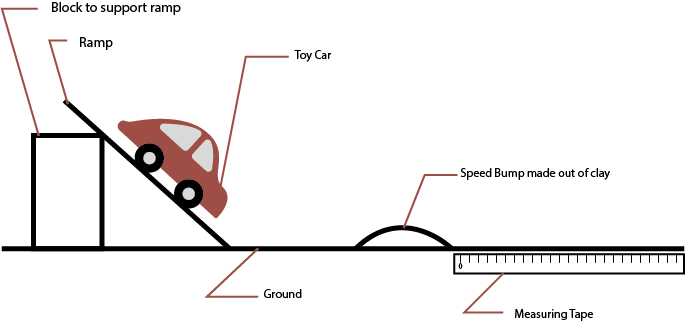
\includegraphics[scale=0.41]{diag.png}
    \caption{Experimental Set-up}
    \label{fig:setup}
  \end{figure}

  \subsubsection{Model}
Our experiment will seek to simulate a speeding car arriving at a speed bump and
consequently slowing down. A toy car will be released and its gravitational
potential energy will convert to kinetic energy (and heat, sound etc.) as it
rolls down. It will then collide with the speed bump and possibly make it over
the speed bump and continue moving to the right in the diagram until it slows
down and stops due to the work done against the car by friction. The speed bump
will be constructed out of clay and its curvature will be modelled after the
speed bump profile being investigated.

The experiment will be recorded by a phone camera and the velocity and
acceleration of the of the vehicle will be interpreted by Tracker and analysed
with Vernier's Logger application. Using this we will be able measure each speed
bump profile and its optimal height using the aforementioned velocity loss to
peak vertical acceleration ratio.

Our experiment will investigate parabolic, sinusoidal, and trapezoidal speed
bumps (or humps), characterised by $p(x) = ax^2$, $s(x) = a\sin(x)$ and $c(x) =
(x-h)^2 + (y - a)^2 = r^2$, where $h,r$ are constants and $a$ is changed to vary
the height of the speed bump. The speed bump is expressed in terms functions for
greater convenience in differentiating to find the gradient at each point and
calculating the normal force of the speed bump on the wheel.

The height of the speed bump will be adjusted in increments of 10\% of the vehicle's
wheel's radius from 0\% to 110\%.

\subsubsection{Apparatus}
\begin{itemize}
  \item Phone Camera
  \item Toy Car
  \item Moulding Clay
  \item Measuring Tape
  \item Rulers (for use in constructing the speed bump)
  \item Ramp and Block
\end{itemize}
\subsection{Safety Precautions and Limitations of Model}
In order to avoid shearing the soft clay speed bump as the vehicle passes and
for the personal safety of us and those around us, the vehicle will be
reasonably lightweight and the height of the ramp will not pass 1.5m.


\end{document}
